\begin{figure}[!htbp]
\begin{center}

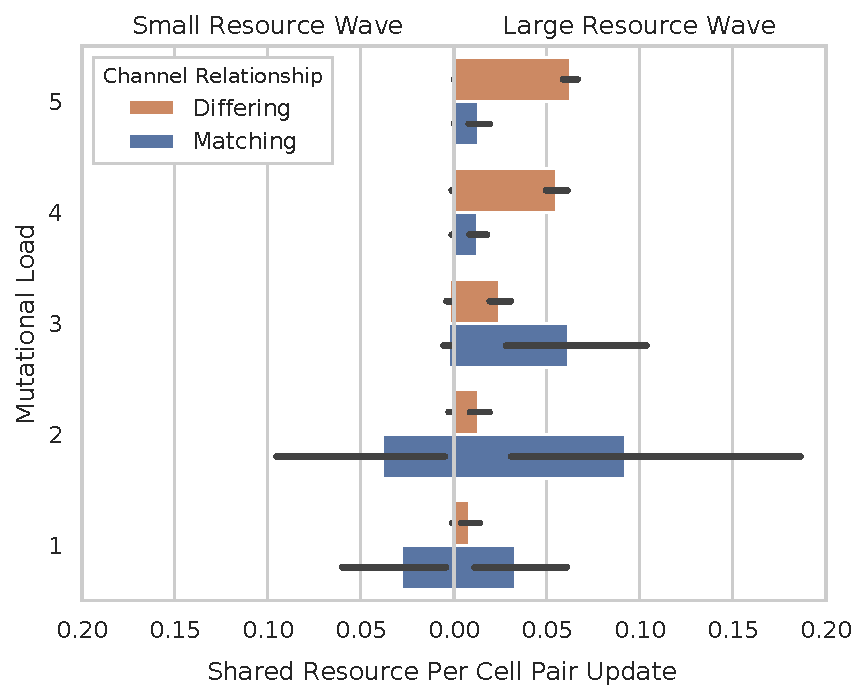
\includegraphics[width=\columnwidth]{title=resource_contributed+_data_hathash_hash=e863a7b8c399f55d+_script_fullcat_hash=ca1d5807a340afac+_source_hash=d53f428-clean+ext=}

\caption{
Resource sharing phenotypes by treatment.
Small resource wave treatments are plotted on the left half of the plot, facing leftwards.
Large resource wave treatments are plotted on the right half of the plot, facing rightwards.
Mutational load increases in the upwards direction.
Bar height represents the mean amount of resource transferred per update per neighboring pair of cells.
Each two-tone pair of bars compares cell pairs with matching channels and cell pairs with differing channels.
Error bars represent 95\% confidence intervals.
} \label{fig:resource_contributed}
\end{center}
\end{figure}
